\documentclass[12pt]{article}
%\documentclass[AER]{AEA}
\usepackage[letterpaper, margin=1in]{geometry}
\usepackage{enumitem}
\usepackage{float}
\setlist[itemize]{leftmargin=*, itemsep=2pt, topsep=2pt, parsep=0pt}
\usepackage{fancyhdr}
\restylefloat{table}
\usepackage{comment}
\usepackage{caption}
\usepackage{graphicx} \usepackage{amsmath,amssymb}
\usepackage[colorlinks=true, allcolors=blue]{hyperref}
\usepackage{natbib}
\usepackage{setspace}
\usepackage{multirow}
\setstretch{1.05}
\title{Local Housing Price Nowcasting}
\author{Vittorio Garavelli, Camilla Nguyen, Lisa Collier \thanks{University of California, Berkeley, Email: vittorio.garavelli@berkeley.edu, lisa.collier@berkeley.edu, cami@berkeley.edu}}

\begin{document}
\maketitle
\vspace{-1.5cm}
\begin{abstract}
\noindent We benchmark four standard predictive approaches --- pooled OLS with metro fixed effects, ARIMA, XGBoost, and a small MLP --- on monthly Zillow Home Value Index (ZHVI) returns for three structurally different US metropolitan areas: San Francisco, Austin, and Cleveland. Predictors come from FRED macroeconomic series and Zillow listing-side variables. Models are trained on pre-2023 data and evaluated on a January~2023--March~2026 test set that covers the post-2022 mortgage-rate shock. We document two patterns. First, no single model wins everywhere: OLS is best in San Francisco, MLP is best in Austin, and ARIMA is best in Cleveland. Second, SHAP attribution on the XGBoost model shows that the most important features differ by metro. We read these results as evidence that, in the United States, both model selection and dominant features are geographically contingent.
\end{abstract}

\pagenumbering{arabic}

\section{Introduction}

Housing markets play a central role in household wealth, local economies, and monetary policy. According to Matteo Iacoviello, housing wealth represents ``one half of household net worth'' \cite{iacoviello2011}, which makes it a determinant of the broader economy: losses in housing wealth can dramatically decrease consumption, with consequences for monetary policy and GDP growth. Because housing amplifies economic expansions and recessions, predicting housing prices in real time has real practical value. However, official indicators such as the Case-Shiller Index and the Federal Housing Finance Agency price index are consistently published with latency, which limits the ability of policymakers, investors, and economists to assess current market conditions.

This work addresses that gap empirically. Nowcasting refers to a framework that attempts to ``estimate complex case counts for a given reporting date, using time series of case reports that are known to be incomplete due to reporting delays'' \cite{mcgough2020}; in our setting it means using real-time indicators to predict the current month's housing price before the official Zillow figure is released. We do not propose a new method. Rather, our goal is to \emph{benchmark} four standard predictive approaches --- a pooled OLS regression with metropolitan fixed effects, a univariate ARIMA model, a gradient-boosted tree model (XGBoost), and a two-layer neural network (MLP) --- on three structurally different US metropolitan areas: San Francisco, California; Austin, Texas; and Cleveland, Ohio.

The questions we ask are descriptive and comparative. \textbf{(i)~Do specific features emerge as the major drivers of monthly housing-price returns, or does the answer depend on the metropolitan area?} \textbf{(ii)~Is model selection itself geographically contingent in the United States --- that is, does the best-performing model differ across structurally different metros, or does one approach dominate everywhere?} The models are trained on pre-2023 data and evaluated on a January~2023--March~2026 test set that covers the post-2022 mortgage-rate-shock regime, providing a demanding out-of-sample comparison.

\section{Literature Review}
\label{sec:lit}

Our empirical design draws on three strands of the housing-forecasting literature: state-level forecastability, predictor heterogeneity across local markets, and the comparison between econometric baselines and machine-learning methods. We first draw on \citet{rapach2009forecasting}, who forecast \textit{state-level} real housing price growth in the United States from 1995 to 2006 using a wide set of state, regional, and national economic predictors. We adopt the same core macroeconomic series (mortgage rate, CPI, unemployment) retrieved from FRED. Their central result is that forecastability differs sharply between \textit{interior} and \textit{coastal} US states: autoregressive and multi-predictor models perform relatively well for many interior states, but all models perform poorly for a group of primarily coastal states that experienced especially strong price growth, suggesting a ``disconnect'' between prices and fundamentals there. We extend the spirit of this comparison to the \textit{metropolitan} level, selecting one coastal market (San Francisco), one Sun Belt market (Austin), and one interior market (Cleveland) to test whether the interior-versus-coastal forecastability gap holds across structurally different metros and into a much later sample period.

We also draw on \citet{kholodilin2014business}, who evaluate a large set of indicators to forecast housing prices and rents across 71 large German cities. Their central finding is that \textit{no single predictor} dominates across all cities and market segments, with the most useful indicators (national business confidence, consumer confidence, price-to-rent ratios) varying by local context. This motivates our use of \textit{both} listing-side variables (new listings, days-pending, price cuts) \textit{and} macroeconomic indicators, as well as our application of SHAP attribution to identify which variables drive the predictions in each metro.

Finally, our choice of competing model architectures is motivated by \citet{plakandaras2015forecasting}, who compare a machine-learning specification (Support Vector Regression with Ensemble Empirical Mode Decomposition) against Random Walk, Bayesian Autoregressive, and Bayesian VAR baselines for the US real house price index, and find that the machine-learning approach substantially outperforms the econometric baselines out of sample. We adopt the same design principle, comparing a linear baseline (OLS), a univariate time-series baseline (ARIMA), a tree-based ensemble (XGBoost), and a small neural network (MLP) on the same test set, but at the metropolitan rather than national level. Our contribution sits at the intersection of these three strands: we implement metro-level housing nowcasting on three structurally different US markets, compare classical econometric and machine-learning models on a common test set, and use SHAP attribution to surface the variables that drive each model's predictions city by city.


\section{Data}
\label{sec:data}

In this research, we use three data sources to build a monthly panel that covers our three pre-selected metropolitan areas. The raw Zillow and national FRED panel spans January~2000 to March~2026. The supervised complete-case sample begins in 2018 because the Zillow listing-side variables are unavailable before then and predictors are lagged. The OLS, XGBoost, and MLP models are trained on 168 complete pre-2023 observations and evaluated on 97 complete test observations (36 in San~Francisco, 36 in Austin, 25 in Cleveland). The ARIMA baseline is estimated separately by metro on the longer target-only ZHVI return history (back to January~2000) and then aligned to the same 97-observation supervised test grid for evaluation.

\subsection{Zillow Home Value Index}

Our first data source is the Zillow Home Value Index (ZHVI). This smoothed and seasonally adjusted variable quantifies the median home value for the middle price tier in each metropolitan area. The indicator is published monthly by Zillow Research and is available from January 2000 onward. We load this data source automatically in our notebook from Zillow's public static CSV URL.

In addition to the Home Value Index, we use three other real-time market activity variables published by Zillow Research: the monthly count of new listings, the median number of days a home sits on the market before going under contract, and the share of active listings that received a price reduction. These three variables impose a time constraint on the continuity of our dataset, as they are only available from 2018 onward. We therefore adjust our sample timeline to begin in that year.

Figure~\ref{fig:zhvi} shows the different paths for housing prices over the entire period in the three metros.

\begin{figure}[!htb]
\centering
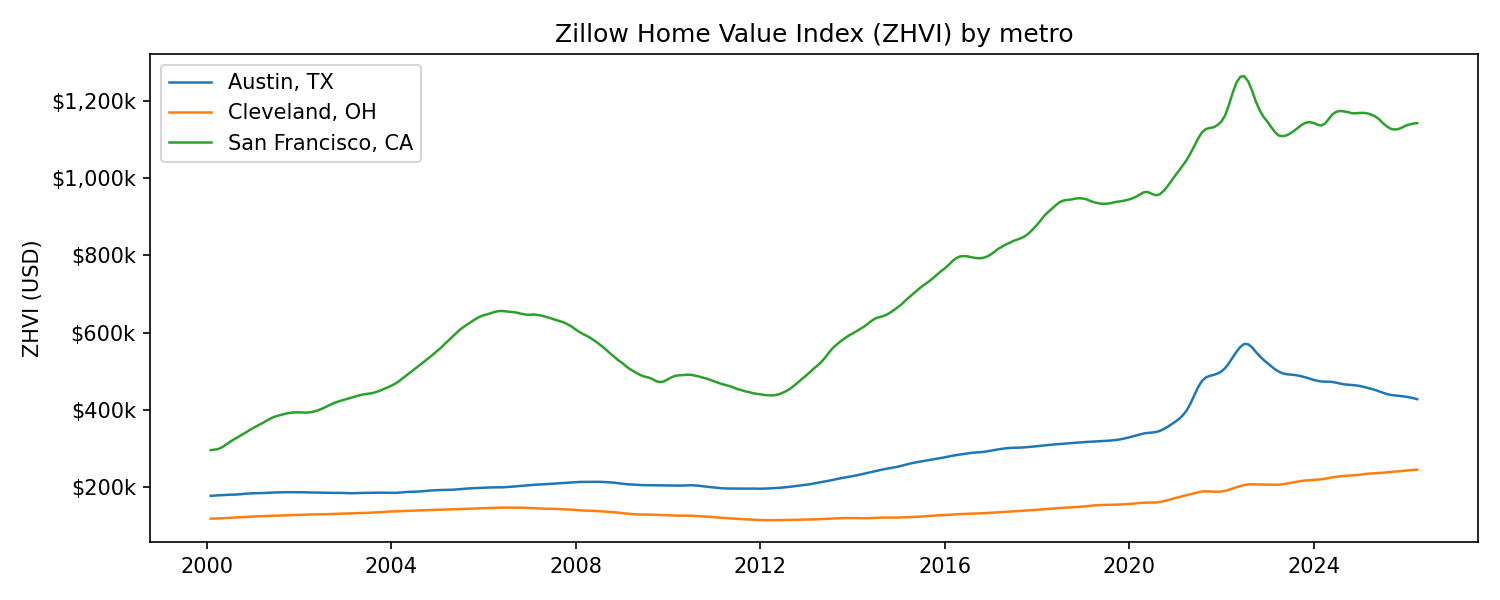
\includegraphics[width=0.68\textwidth]{zhvi_levels.png}
\caption{Zillow Home Value Index, by metro, January 2000 to March 2026. San Francisco and Austin experience steep price growth and increased volatility compared to Cleveland, whose path is more steady and less volatile.}
\label{fig:zhvi}
\end{figure}


\subsection{National Macroeconomic Indicators}

We selected five national economic indicators from the Federal Reserve Bank of St. Louis (FRED). These time series capture the key macroeconomic mechanisms through which monetary policy and credit conditions react to and affect local housing markets. First, the 30-year mortgage rate proxies buyer affordability and therefore housing demand. Second, the national unemployment rate reports labor market conditions. Third, the Consumer Price Index measures inflation and captures fluctuations in the real cost of housing. Fourth, housing starts measure new construction activity, which serves as a proxy for supply-side conditions. Finally, the St. Louis Fed Financial Stress Index captures credit-market conditions beyond the policy rate. We convert the weekly series into monthly averages to align them with the Zillow and unemployment indicators.

\subsection{Metro-Level Unemployment}

To adjust our approach to the metropolitan level, we use monthly, seasonally adjusted series that capture local labor market conditions that the national indicators cannot. Specifically, we include metro-specific unemployment series, as additional independent variables, from the Bureau of Labor Statistics Local Area Unemployment Statistics (LAUS). We retrieve them via FRED: series \texttt{SANF806URN} for San~Francisco, \texttt{AUST448URN} for Austin, and \texttt{CLEV439URN} for Cleveland.

Figure~\ref{fig:unrate} displays the unemployment trends for all three metros alongside the national average rate, demonstrating the differences in their labor markets over the sample period

\begin{figure}[!htb]
\centering

\includegraphics[width=0.68\textwidth]{unrate_metro.png}
\caption{Metro-level unemployment rates (LAUS, seasonally adjusted) versus the national unemployment rate (dashed), January 2000 to March 2026. San Francisco displays greater cyclical movements, whereas Cleveland sustains a steady but higher level of unemployment.}
\label{fig:unrate}
\end{figure}


\subsection{Sample Construction and Cleaning}

We merge the three data sources into a single dataframe in which each row corresponds to one observation per city per month, broadcasting the national macroeconomic indicators across all metros. Because the three Zillow listing-side variables are missing before 2018, we drop rows with missing values, which constrains the supervised modeling sample to 2018 onward. After cleaning, the supervised complete-case panel contains 168 training observations (pre-2023) and 97 test observations across the three metros (36 in San~Francisco, 36 in Austin, 25 in Cleveland). The ARIMA baseline does not require the lagged exogenous predictors, so it is estimated on the longer per-metro target-only history (back to 2000) and then evaluated on the same 97-observation supervised test grid for a strictly same-sample comparison. Figure~\ref{fig:missing} confirms that the Zillow listing-side variables are what constrain the start date of the supervised training window.

The smaller Cleveland test sample (25 observations versus 36 for the other two metros) is not driven by the Zillow listing-side variables. It reflects the fact that the extracted Cleveland LAUS metro unemployment series ends in December~2024 in our data pull, while the Zillow and national FRED series extend through March~2026. After the one-month lag is applied to \texttt{d\_unrate\_metro}, the last test month in which Cleveland passes the complete-case mask is January~2025.

\subsection{2024 ACS Variables (Descriptive Only)}

We also downloaded 2024 ACS 5-year metro-level variables --- median household income, median home value, and the rental vacancy rate --- for descriptive context. We do \emph{not} include them in the final model matrix because they are time-invariant within each of the three metros and are therefore perfectly collinear with the full set of metro fixed effects. The metro fixed effects already absorb these structural cross-metro differences (price level, income, vacancy regime), so adding the ACS variables would simply duplicate the dummies and make the design matrix rank-deficient.

\begin{figure}[!htb]
\centering

\includegraphics[width=0.68\textwidth]{missingness.png}
\caption{Share of missing observations per variable by year. Dark cells represent complete data; light cells indicate missing  values. The Zillow listing-side variables (new listings, days  pending, price cuts) are missing before 2018, which determines the effective start of the modeling sample.}
\label{fig:missing}
\end{figure}


Table~\ref{tab:summary} provides summary statistics of the relevant variables in the modeling sample by metropolitan area.

\begin{table}[h]
\centering
\small
\caption{Summary statistics by metropolitan area.
ZHVI is presented in thousands of US dollars. Log return is the monthly log return of ZHVI. Metro unemployment is the LAUS seasonally-adjusted rate expressed as a percentage. Listing-side variables (new listings, price cuts) pertain to the period beginning in 2018, when Zillow first publishes them. ZHVI and log return cover the full 2000--2026 window (315~observations per metro). The metro unemployment series cover the full window for San~Francisco and Austin (313~observations) and 2000--2024 for Cleveland (300~observations), reflecting the earlier end-date of the Cleveland LAUS pull.}
\label{tab:summary}
\begin{tabular}{llcccc}
\hline
Metro & Variable & Mean & Std & Min & Max \\
\hline
\multirow{5}{*}{San Francisco}
  & ZHVI (\$000s)        & 716.2  & 275.3 & 294.9  & 1264.8 \\
  & Log return           & 0.0043 & 0.0093 & -0.0234 & 0.0270 \\
  & Metro unemployment   & 5.37  & 2.25  & 2.3    & 13.9   \\
  & New listings         & 3323  & 972   & 1426   & 5136   \\
  & Price cuts (\%)      & 0.151 & 0.047 & 0.061  & 0.262  \\
\hline
\multirow{5}{*}{Austin}
  & ZHVI (\$000s)        & 279.1  & 110.9 & 176.3  & 570.4  \\
  & Log return           & 0.0028 & 0.0081 & -0.0216 & 0.0509 \\
  & Metro unemployment   & 4.50  & 1.48  & 2.4    & 11.5   \\
  & New listings         & 2957  & 810   & 1567   & 4835   \\
  & Price cuts (\%)      & 0.222 & 0.078 & 0.044  & 0.370  \\
\hline
\multirow{5}{*}{Cleveland}
  & ZHVI (\$000s)        & 148.4  & 35.5  & 112.9  & 244.5  \\
  & Log return           & 0.0023 & 0.0046 & -0.0083 & 0.0179 \\
  & Metro unemployment   & 5.57  & 1.91  & 2.1    & 20.6   \\
  & New listings         & 2440  & 638   & 1326   & 3677   \\
  & Price cuts (\%)      & 0.189 & 0.039 & 0.112  & 0.273  \\
\hline
\multicolumn{6}{l}{\footnotesize Note: 30-year mortgage rate is national 
(mean 5.21\%, std 1.39\%, range 2.68--8.52\%) and} \\
\multicolumn{6}{l}{\footnotesize identical across metros; reported once 
here to avoid repetition.} \\
\end{tabular}
\end{table}

\section{Empirical Strategy}
\label{sec:method}


\subsection{Target Variable}

We model the monthly log return of ZHVI rather than the raw price level or the dollar change:

$$y_t = \ln\!\left(\frac{\text{ZHVI}_t}{\text{ZHVI}_{t-1}}\right)$$

We orient our analysis toward log returns for three main reasons. First, because we estimate OLS and ARIMA models, raw home values exhibiting an upward trend over time would have violated the stationarity requirement of these methods. Log returns instead fluctuate around a stable mean and are more suitable for statistical modeling. Second, log returns put the three cities on a comparable scale (a 0.5\% monthly change represents the same effect in San Francisco and in Cleveland, whereas a \$5{,}000 change does not), which makes them comparable across our three local areas. Third, log returns are the standard unit used in economic research on rates of appreciation. Throughout this paper we use the term ``nowcasting'' in its applied sense in housing economics: predicting the current month's ZHVI return using indicators available at the start of that month, before the official Zillow figure is published.



\subsection{Feature Engineering}

\subsubsection{Stationarity Transforms}

To satisfy the stationarity requirements of our predictive models, we apply transformations to our raw economic series measured in levels. The transformations applied to each variable before estimation are as follows:

\begin{itemize}
    \item We first-difference the mortgage rate, the national unemployment rate, and the metro unemployment rate. The reason is that, to analyze housing demand, we need to observe whether rates went up or down; their respective levels are not directly relevant.
    \item We log-transform new listings, housing starts, and days on market to compress the right tail of their distributions and stabilize variance across the sample.
    \item We express CPI as a 12-month log change, which is the standard economic definition of the inflation rate.
    \item The financial stress index and the share of price cuts are already stable, so we keep them as-is.
\end{itemize}

Figure~\ref{fig:stationary} demonstrates the impact of these transformations on the two selected series.

\begin{figure}[!htb]
\centering

\includegraphics[width=0.68\textwidth]{stationarity.png}
\caption{Mortgage rate (left) vs. transformed series (right) for mortgage rate and CPI, taking Austin as the selected metropolitan. The first difference takes care of the trend in the mortgage rate; the year-over-year percentage change in the log level transforms the CPI into a stationary inflation rate.}
\label{fig:stationary}
\end{figure}

\subsubsection{Lagging Predictor Variables}

To ensure that the model only uses data that was available at the start of the prediction month, we shift the eight leading indicators (the differenced mortgage rate, the two unemployment changes, the three Zillow listing-side variables, the financial-stress index, and the log change in housing starts) back by one month. This eliminates look-ahead bias on those eight series: a change in the mortgage rate in March is treated as affecting buyer behavior in April and beyond, but not in March. Had we used same-month values, our estimates would be biased through data leakage.

CPI year-over-year inflation (\texttt{cpi\_yoy}) is the only feature kept contemporaneous with the prediction month. CPI YoY is a 12-month moving signal and is therefore highly persistent, so the difference between \texttt{cpi\_yoy}\textsubscript{$t$} and \texttt{cpi\_yoy}\textsubscript{$t-1$} is economically negligible; we treat it as the inflation regime indicator at month $t$ rather than as a leading indicator that requires a lag.

\subsubsection{Metro Fixed Effects}

We create three binary indicators (one per city) from the metropolitan area identifiers, allowing each pooled model to use a separate baseline intercept that absorbs time-invariant differences in price level, income, and supply structure across the three metros.

\subsection{Train / Test Split}

We use a single chronological split: observations through December 2022 form the training set, and observations from January 2023 onward form the test set. A chronological split is necessary because a random split would let the model use future observations to predict past ones, producing optimistic, biased performance estimates. We set the split point to December 2022 specifically so that the test period covers the regime immediately following the largest rise in mortgage rates in four decades, ensuring that the training and test periods operate under substantially different macroeconomic conditions.

Figure~\ref{fig:split} gives the complete-case coverage by metro for both training and test datasets.


\begin{figure}[!htb]
\centering

\includegraphics[width=0.68\textwidth]{split_coverage.png}
\caption{Complete observation coverage in each metropolitan area. Blue denotes training observations (till December~2022); red denotes test observations (January~2023 onwards). Cleveland contributes fewer complete test observations than San~Francisco or Austin because the extracted Cleveland LAUS metro-unemployment series ends in December~2024, while the Zillow and national FRED series extend through March~2026.}
\label{fig:split}
\end{figure}


\subsection{Models}

We focus on four predictive models of increasing complexity. All models are evaluated on the same test set.

\textbf{OLS Baseline.} Our first model is a pooled ordinary least squares regression estimated across all three cities simultaneously. Metro fixed effects enter as additive intercept shifts. OLS serves as the linear baseline.

\textbf{ARIMA Baseline.} Our second model is an AIC-selected ARIMA model estimated separately for each city (yielding ARIMA(4,\,0,\,9) for Austin, ARIMA(1,\,0,\,7) for San Francisco, and ARIMA(9,\,0,\,7) for Cleveland). This model only uses the target variable's own history and no external economic data. The role of this model is to answer the question: how much of housing-price movement is just momentum? If this benchmark cannot be beaten by models with exogenous regressors, the additional data sources are adding noise rather than signal.

\textbf{XGBoost.} Our third model is a gradient-boosted tree model. XGBoost builds an ensemble of shallow decision trees sequentially, each one learning from the mistakes of the previous one. This model can capture non-linear associations between variables. We chose hyperparameters conservatively to limit overfitting given the small training sample.

\textbf{MLP.} Our fourth and final model is a small two-layer neural network with 16 and 8 hidden units and ReLU activations. All inputs and the target variable are standardized before training to ensure that the optimizer converges effectively. Strong L2 regularization is applied to prevent the network from extrapolating aggressively to test-period inputs that lie outside the training distribution.

\subsection{Evaluation Metrics}

We use two metrics to evaluate all four models. First, we report the mean absolute error on log returns, which is directly comparable across cities with different price levels. Second, we report a dollar MAE that translates prediction errors into dollars per month:

$$\text{Dollar MAE} = \frac{1}{n}\sum_{t} \text{ZHVI}_{t-1} \cdot
|\exp(\hat{y}_t) - \exp(y_t)|$$

The dollar MAE makes the economic magnitude of prediction errors concrete and interpretable. We additionally apply SHAP feature attributions to the XGBoost model to understand which variables drive predictions in each city on the test set.


\section{Results}
\label{sec:results}

\subsection{Model Comparison}

We evaluate all four of our models on the same complete-case test set, which runs from January~2023 to March~2026. After cleaning, we are left with 36 test observations in San~Francisco and Austin and 25 in Cleveland, applied uniformly to all four models. The smaller Cleveland count reflects the fact that the extracted Cleveland LAUS metro unemployment series ends in December~2024, while the Zillow and national FRED series extend through March~2026; once the one-month lag is applied to \texttt{d\_unrate\_metro}, Cleveland's last complete-case test month is January~2025. We report the two metrics defined in Section~\ref{sec:method}: the mean absolute error in log returns and the dollar-denominated MAE.

\begin{table}[!htb]
\centering
\caption{Dollar MAE by model and metro (USD per month, test period: 2023-01 to 2026-03). Bold indicates the best performance for each metro in the row.}
\label{tab:dollar_mae}
\begin{tabular}{lrrrr}
\hline
Metro & OLS & ARIMA(AIC) & XGBoost & MLP(16,8) \\
\hline
San Francisco, CA & \textbf{\$3{,}898} & \$5{,}660 & \$4{,}210 & \$5{,}219 \\
Austin, TX        & \$2{,}574 & \$2{,}371 & \$3{,}494 & \textbf{\$2{,}286} \\
Cleveland, OH     & \$748     & \textbf{\$491} & \$549 & \$1{,}064 \\
\hline
\end{tabular}
\end{table}

Figure~\ref{fig:maebar} provides the dollar MAE results for
all model-metro pairings.

\begin{figure}[!htb]
\centering

\includegraphics[width=0.68\textwidth]{mae_dollars_bar.png}
\caption{Dollar MAE for metro areas and models (test period: 
2023-01 to 2026-03). The lower bars represent better forecasting performance. Not one model stands out as best in all markets.}
\label{fig:maebar}
\end{figure}


\begin{table}[!htb]
\centering
\caption{Mean absolute error on log returns by model and metro (test period: 2023-01 to 2026-03). Bold indicates the best performance for each metro in the row.}
\label{tab:logmae}
\begin{tabular}{lrrrr}
\hline
Metro & OLS & ARIMA(AIC) & XGBoost & MLP(16,8) \\
\hline
San Francisco, CA & \textbf{0.00339} & 0.00497 & 0.00368 & 0.00455 \\
Austin, TX        & 0.00555 & 0.00518 & 0.00748 & \textbf{0.00488} \\
Cleveland, OH     & 0.00339 & \textbf{0.00226} & 0.00253 & 0.00487 \\
\hline
\end{tabular}
\end{table}


Figure~\ref{fig:preds} plots the estimated log returns for all four models compared to the actual time series in the test period.

\begin{figure}[!htb]
\centering

\includegraphics[width=0.68\textwidth]{predictions_vs_actual.png}
\caption{Estimated vs. Actual Monthly Log Returns of ZHVI 
in the Test Period (Jan. 2023 to Mar. 2026). The black line is the actual time series, while the colored lines represent model forecasts.}
\label{fig:preds}
\end{figure}


Our results show that no single model wins across all three markets. In San~Francisco, the pooled OLS model produces the best performance at \$3{,}898 per month, outperforming both non-linear models. In Austin, the MLP achieves the lowest dollar MAE at \$2{,}286 per month, with ARIMA a close second at \$2{,}371 per month --- a margin of less than \$100, so the MLP's edge over the pure time-series benchmark is small. In Cleveland, the MLP produces its worst performance, with a dollar MAE of \$1{,}064 per month, while ARIMA is the most convincing model for that metro at \$491 per month. Overall, these patterns demonstrate that model performance is geographically contingent.

\subsection{SHAP Feature Importance}

To add precision to our XGBoost results, we compute SHAP (SHapley Additive exPlanations) values over the test set and average contributions by metro. Three distinct patterns emerge. In \textbf{Cleveland}, \texttt{price\_cuts} carries the most weight (mean $|\text{SHAP}|=0.0039$), followed by \texttt{d\_log\_days\_pending} ($0.0011$), while housing starts are nearly irrelevant ($0.0002$); this is consistent with a friction-sensitive, supply-constrained market in which transaction signals dominate. In \textbf{Austin}, \texttt{price\_cuts} alone is roughly five times more influential than any other variable and accounts for much of the predictive advantage of listing-side data over purely macro-driven models, which fits Austin's volatile, demand-driven market where seller behavior is more informative than national macro series. In \textbf{San Francisco}, the metro indicator carries most of the weight ($0.0028$), followed by \texttt{price\_cuts} ($0.0018$) and \texttt{d\_mortgage30} ($0.0011$), suggesting that structural characteristics of the Bay Area (income distribution, price level) explain more of the monthly variation than any single time-varying indicator.

Table~\ref{tab:shap} lists the mean absolute SHAP values for the most important features per metropolitan area.

\begin{table}[!htb]
\centering
\caption{Mean absolute SHAP values by feature and metro 
(XGBoost, test set). Higher values indicate greater average 
contribution to the model's prediction.}
\label{tab:shap}
\begin{tabular}{lrrr}
\hline
Feature & San Francisco & Austin & Cleveland \\
\hline
\texttt{price\_cuts}           & 0.00180 & \textbf{0.00662} & \textbf{0.00391} \\
\texttt{metro\_San Francisco}  & \textbf{0.00279} & 0.00125 & 0.00122 \\
\texttt{d\_mortgage30}         & 0.00114 & 0.00088 & 0.00084 \\
\texttt{d\_log\_days\_pending} & 0.00086 & 0.00067 & 0.00110 \\
\texttt{d\_log\_new\_listings} & 0.00085 & 0.00063 & 0.00081 \\
\texttt{stlfsi}                & 0.00078 & 0.00071 & 0.00053 \\
\texttt{cpi\_yoy}              & 0.00046 & 0.00098 & 0.00053 \\
\texttt{d\_log\_houst}         & 0.00022 & 0.00020 & 0.00019 \\
\hline
\end{tabular}
\end{table}

\subsection{OLS Regression Table}

Table~\ref{tab:ols} reports the pooled OLS estimates ($N=168$, training sample 2018-01 to 2022-12). HAC (Newey--West, 3 lags) standard errors. The constant is omitted because the three metro dummies span the all-ones vector and serve as per-metro intercepts.

\begin{table}[!htb]
\centering
\small
\caption{Pooled OLS estimates. Dependent variable: monthly log return of ZHVI. ${}^{***}p<0.01$, ${}^{*}p<0.10$.}
\label{tab:ols}
\begin{tabular}{lrrr}
\hline
Predictor & Coef. & Std. Err. & $p$-value \\
\hline
\multicolumn{4}{l}{\textit{Time-varying predictors (lagged one month except CPI YoY)}} \\
\texttt{d\_mortgage30}        &  $0.0081^{***}$  & 0.002 & 0.000 \\
\texttt{d\_unrate\_nat}       &  $0.0005$        & 0.001 & 0.573 \\
\texttt{d\_unrate\_metro}     & $-0.0009$        & 0.001 & 0.347 \\
\texttt{d\_log\_houst}        & $-0.0068$        & 0.004 & 0.131 \\
\texttt{d\_log\_new\_listings}& $-0.0099^{*}$    & 0.005 & 0.062 \\
\texttt{d\_log\_days\_pending}&  $0.0032$        & 0.006 & 0.584 \\
\texttt{price\_cuts}          & $-0.1647^{***}$  & 0.015 & 0.000 \\
\texttt{stlfsi}               & $-0.0021^{***}$  & 0.001 & 0.006 \\
\texttt{cpi\_yoy}             & $-0.1010^{***}$  & 0.032 & 0.001 \\
\hline
\multicolumn{4}{l}{\textit{Metro fixed effects (per-metro intercepts)}} \\
\texttt{metro\_Austin}        &  $0.0439^{***}$  & 0.004 & 0.000 \\
\texttt{metro\_Cleveland}     &  $0.0380^{***}$  & 0.003 & 0.000 \\
\texttt{metro\_San~Francisco} &  $0.0296^{***}$  & 0.003 & 0.000 \\
\hline
$N$ & \multicolumn{3}{l}{168} \\
$R^{2}$ & \multicolumn{3}{l}{0.746} \\
Adj.~$R^{2}$ & \multicolumn{3}{l}{0.728} \\
Durbin--Watson & \multicolumn{3}{l}{0.637} \\
\hline
\end{tabular}
\end{table}

\subsection{Model Interpretability}

The four models differ in how much they support an economic reading of the predictions. \textbf{ARIMA} contains no exogenous regressors: its AR and MA coefficients describe the internal time-series structure of returns but cannot speak to which economic variables drive prices. The \textbf{MLP} is non-interpretable by design --- with ReLU activations and L2 regularization, individual weights have no economic meaning without post-hoc attribution, which we did not apply. \textbf{XGBoost} is interpretable in the sense we want via the SHAP attribution reported above (Table~\ref{tab:shap}). \textbf{OLS} is the only model whose coefficients are in principle interpretable as the marginal effect of each predictor on the log return. However, several diagnostics suggest reading them as descriptive partial correlations rather than causal estimates:

\begin{itemize}
    \item \textbf{Wrong-signed mortgage rate.} The estimated coefficient is positive ($\hat{\beta}_{\text{mortgage}} = +0.0081$), the opposite of what housing-demand theory predicts; this is most plausibly a confounding artefact of the post-COVID regime in which rates and prices both rose.
    \item \textbf{Statistical caveats.} Three regressors are borderline non-stationary by ADF (\texttt{d\_mortgage30} $p=0.063$, \texttt{d\_log\_days\_pending} $p=0.076$, \texttt{price\_cuts} $p=0.055$); the Durbin--Watson statistic of $0.64$ indicates strong positive residual autocorrelation; and national and metro unemployment have variance inflation factors near 8. Together these mean coefficients are inefficient and standard errors are too tight even with HAC correction.
    \item \textbf{Pooled across metros.} Each $\hat{\beta}$ is the average effect across San Francisco, Austin, and Cleveland; the pooled estimate masks any slope heterogeneity (this shows up indirectly through the per-metro intercepts but not through metro-specific slopes).
\end{itemize}

\section{Discussion}

While the goal of our paper was not to reproduce the findings of any paper mentioned in the Literature Review, our results follow the same patterns. In particular, our findings echo the core result of \citet{kholodilin2014business}, who document that no single \emph{predictor} dominates across all German cities; we observe an analogous pattern for \emph{model architectures}, with no single nowcasting model outperforming the others across all three metros. Instead, each model outperforms the others in a specific geographical area. We therefore argue that the optimal model type depends on the structural and macroeconomic characteristics under which a local housing market operates. Our choice of metropolitan areas was specifically designed to highlight this aspect and constitutes a core strength of our research.

\subsection{Limitations}
Several limitations constrain our findings. First, the missingness of the Zillow listing-side variables before 2018 reduces the usable training window, leaving us with only 186 complete observations for three of the four models. This small sample raises overfitting risk for XGBoost and MLP; we mitigate this with conservative hyperparameters (shallow trees and heavy L2 regularization), but a longer historical record would allow these models to better exploit their capacity. Second, we estimate the ARIMA models once on the training series and produce predictions for the full test period without updating; a rolling re-estimation scheme would more accurately reproduce real-time conditions and would likely improve ARIMA performance.

\subsection{Policy Implications}
Despite these limitations, our findings offer practical implications for real-time housing market analysis. In particular, the strong performance of listing-side data across all three cities suggests that publicly available Zillow indicators can significantly improve price nowcasting. Additionally, for policy purposes, our research suggests that locally calibrated nowcasting models will outperform any attempt at a universal model.

\section{Conclusion}
In conclusion, this paper contributes to a growing literature on housing market nowcasting by demonstrating that model selection and feature importance are geographically contingent rather than universal. Drawing on past research, our paper extends prior findings along two dimensions. First, it develops the framework at the metropolitan level using real-time listing-side data. Second, it applies SHAP feature attribution to quantify precisely which variables drive each model's performance in each local market. Future work could extend this framework by incorporating higher-frequency data, applying rolling re-estimation to the ARIMA baseline, or expanding the metro sample to test whether the geographic heterogeneity we document generalizes beyond our three chosen markets.

\section{AI Usage Disclosure}

In compliance with course policy, we disclose how artificial intelligence was used during this project.

\textbf{Tools.} We used Anthropic's Claude (Opus 4.6 Max and Opus 4.7 Max) as a coding assistant, accessed through the Claude Code command-line interface (\href{https://github.com/anthropics/claude-code}{github.com/anthropics/claude-code}). No other LLMs were used.

\textbf{Tasks.} The model was used in support of code quality, not in framing the research question or drawing economic conclusions. Concretely, we used it to brainstorm potential weaknesses in our design (look-ahead bias, sample-size constraints, residual autocorrelation); to review notebook cells for logic errors and incorrect API use (pandas, statsmodels, scikit-learn, XGBoost); to rewrite verbose code into shorter idiomatic forms; to enforce a consistent visual style across all figures; and to parameterize the train/test boundary and seed (\texttt{SEED = 0}) for reproducibility.

\textbf{Skills and agents.} We invoked reusable prompts and review agents from two open-source collections of \texttt{skill.md} and \texttt{agent.md} files: the Everything Claude Code plugin (\href{https://github.com/affaan-m/everything-claude-code}{github.com/affaan-m/everything-claude-code}) and Scientific Agent Skills (\href{https://github.com/K-Dense-AI/scientific-agent-skills}{github.com/K-Dense-AI/scientific-agent-skills}). No agent had autonomous authority; every suggested change was reviewed manually.

\textbf{Verification.} We treated AI output as proposals: every suggested edit was read line by line, the notebook was re-run end-to-end after each substantive change, and all numerical results were inspected for plausibility against the simple baselines.

{\footnotesize
\setstretch{1.0}
\setlength{\bibsep}{2pt}
\bibliography{Bibliography}
\bibliographystyle{plainnat}}

\end{document}